% !TeX spellcheck = cs_CZ
{\tikzset{external/prefix={tikz/FYZII/}}
 \tikzset{external/figure name/.add={ch35_}{}}
%---------------------------------------------------------------------------------------------------
% file fey2ch35.tex
%---------------------------------------------------------------------------------------------------
%=========================== Kapitola Paramagnetizmus a magnetická rezonance =======================
\chapter{Paramagnetizmus a magnetická rezonance}\label{fyz:IIchapXXXV}
\minitoc
  \section{Kvantové magnetické stavy}\label{fyz:IIchapXXXVsecI}
  \section{Sternův-Gerlachův pokus}\label{fyz:IIchapXXXVsecII}
  \section{Rabiho metoda molekulového svazku}\label{fyz:IIchapXXXVsecIII}
  \section{Paramagnetizmus makroskopických látek}\label{fyz:IIchapXXXVsecIV}
  \section{Chlazení pomocí adiabatické demagnetizace}\label{fyz:IIchapXXXVsecV}
  \section{Jaderná magnetická rezonance}\label{fyz:IIchapXXXVsecVI}
  \section{Příklady a cvičení}\label{fyz:IIchapXXXVsecVII}

    \begin{figure}[ht!] %\ref{fyz_fig846}
      \centering
      \begin{tabular}{c}
        \subfloat[ ]{\label{fyz_fig846a}
          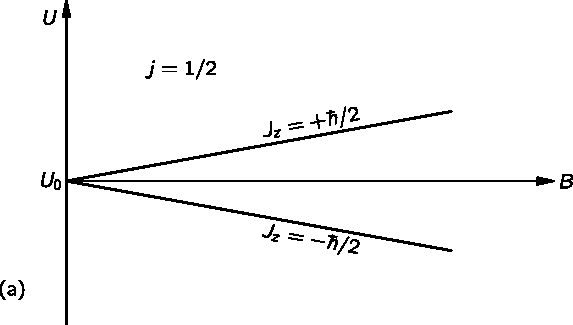
\includegraphics[width=0.7\linewidth]{fyz_fig846a.pdf}}               \\
        \subfloat[ ]{\label{fyz_fig846b}
          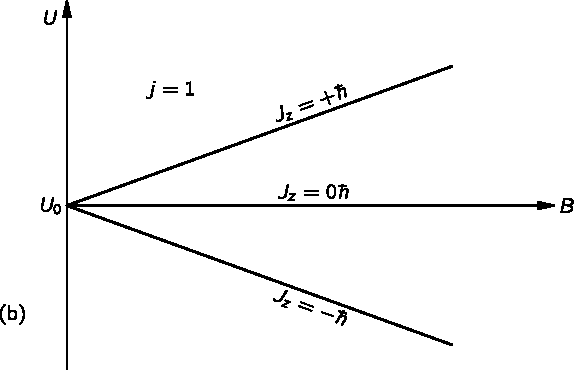
\includegraphics[width=0.7\linewidth]{fyz_fig846b.pdf}}               \\
        \subfloat[ ]{\label{fyz_fig846c}
          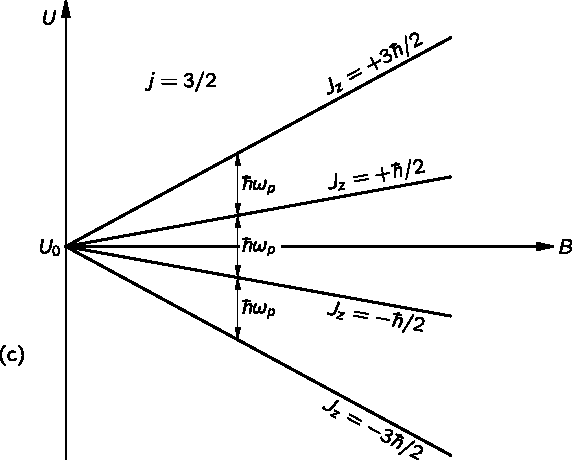
\includegraphics[width=0.7\linewidth]{fyz_fig846c.pdf}}
      \end{tabular}
      \caption{
               (\cite[s.~748]{Feynman02})}
      \label{fyz_fig846}
    \end{figure}

    \begin{figure}[ht!] %\ref{fyz_fig847}
      \centering
      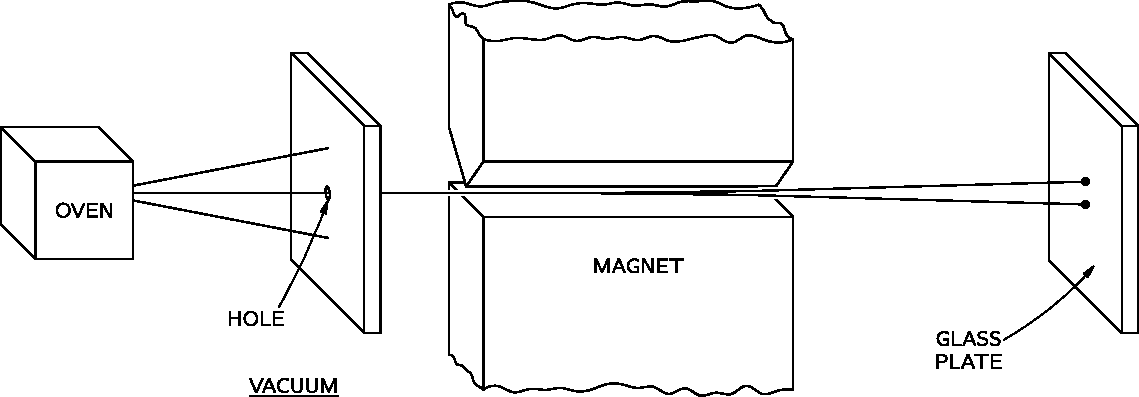
\includegraphics[width=0.7\linewidth]{fyz_fig847.pdf}
      \caption{
               (\cite[s.~707]{Feynman02})}
      \label{fyz_fig847}
    \end{figure}

    \begin{figure}[ht!] %\ref{fyz_fig848}
      \centering
      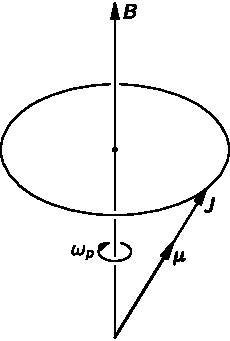
\includegraphics[width=0.7\linewidth]{fyz_fig848.pdf}
      \caption{
               (\cite[s.~707]{Feynman02})}
      \label{fyz_fig848}
    \end{figure}

    \begin{figure}[ht!] %\ref{fyz_fig849}
      \centering
      \begin{tabular}{c}
        \subfloat[ ]{\label{fyz_fig849a}
          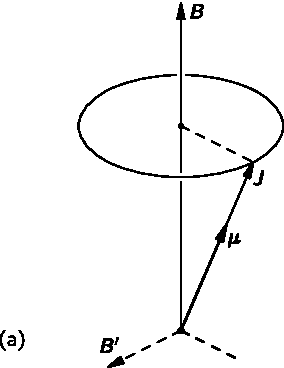
\includegraphics[width=0.7\linewidth]{fyz_fig849a.pdf}}               \\
        \subfloat[ ]{\label{fyz_fig849b}
          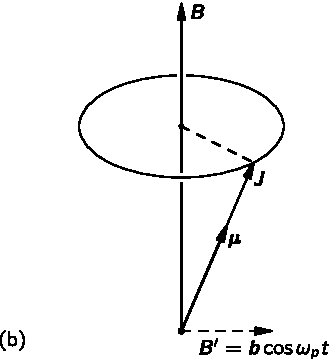
\includegraphics[width=0.7\linewidth]{fyz_fig849b.pdf}}
      \end{tabular}
      \caption{
               (\cite[s.~748]{Feynman02})}
      \label{fyz_fig849}
    \end{figure}

    \begin{figure}[ht!] %\ref{fyz_fig850}
      \centering
      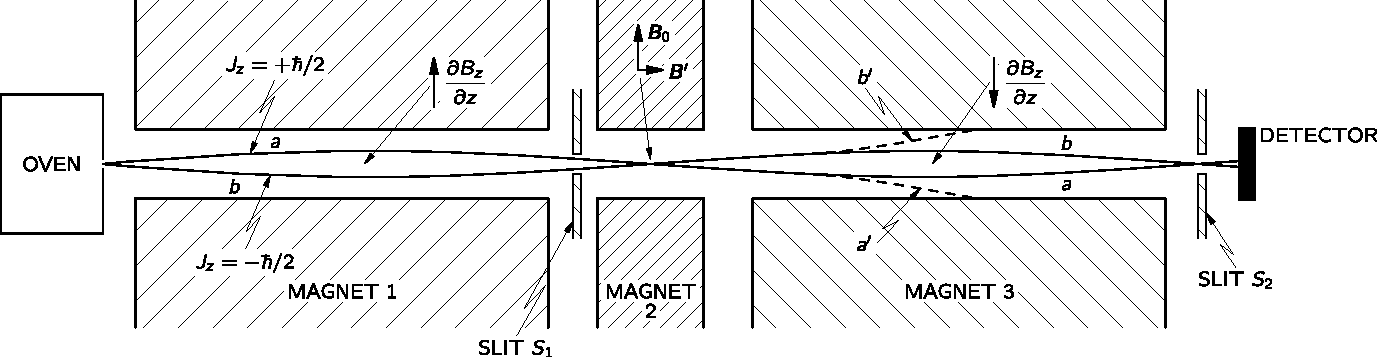
\includegraphics[width=0.7\linewidth]{fyz_fig850.pdf}
      \caption{
               (\cite[s.~707]{Feynman02})}
      \label{fyz_fig850}
    \end{figure}

    \begin{figure}[ht!] %\ref{fyz_fig851}
      \centering
      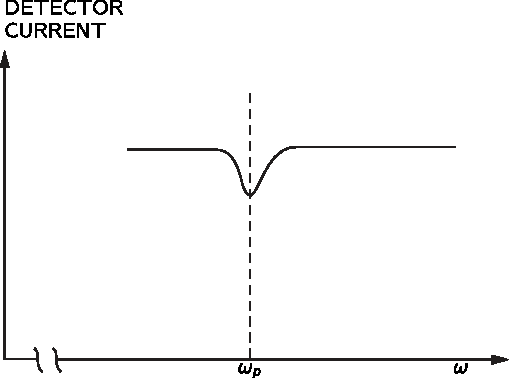
\includegraphics[width=0.7\linewidth]{fyz_fig851.pdf}
      \caption{
               (\cite[s.~707]{Feynman02})}
      \label{fyz_fig851}
    \end{figure}

    \begin{figure}[ht!] %\ref{fyz_fig852}
      \centering
      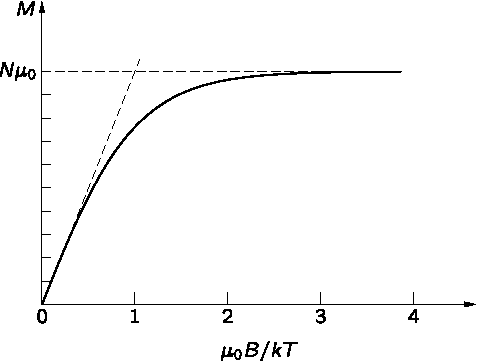
\includegraphics[width=0.7\linewidth]{fyz_fig852.pdf}
      \caption{
               (\cite[s.~707]{Feynman02})}
      \label{fyz_fig852}
    \end{figure}

    \begin{figure}[ht!] %\ref{fyz_fig853}
      \centering
      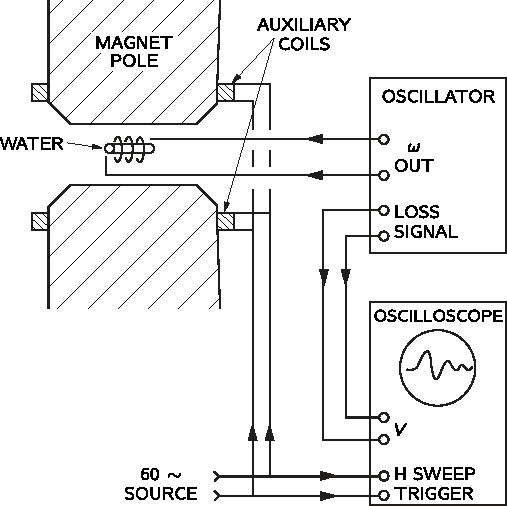
\includegraphics[width=0.7\linewidth]{fyz_fig853.pdf}
      \caption{
               (\cite[s.~707]{Feynman02})}
      \label{fyz_fig853}
    \end{figure}
    
} %tikzset
%---------------------------------------------------------------------------------------------------
\printbibliography[title={Seznam literatury},heading=subbibliography]
\addcontentsline{toc}{section}{Seznam literatury}